\documentclass[a4paper,12pt]{scrreprt}
    %% Used for changing geometry of the page
    %% Cover page text cannot overlay cover sketching/style 
    %% https://ctan.org/pkg/geometry?lang=en
\usepackage{geometry}
    %% Changes language of some packages protocols
    %% e.g., when captioning images: Figure 1. -> Figura 1.
    %% https://ctan.org/pkg/babel?lang=en
\usepackage[portuguese]{babel}
    %% Used for special fonts
    %% Cannot be compiled with pdflatex
    %% https://ctan.org/pkg/fontspec?lang=en
\usepackage{fontspec}
    %% Arial FONT
    \setmainfont{Arial}

    %% More colors and color options
    %% https://ctan.org/pkg/xcolor?lang=en
    %% https://ctan.org/pkg/colortbl?lang=en
\usepackage{xcolor,colortbl}
    %% More tabular options, like dashed/dotted lines
    %% https://ctan.org/pkg/arydshln?lang=en
\usepackage{arydshln}
    %% List of acronyms
    %% https://ctan.org/pkg/nomencl?lang=en
\usepackage[intoc]{nomencl}
    %% Must be called to init nomencl environment  
    \makenomenclature
    %% More images options/settings
    %% https://ctan.org/pkg/graphicx?lang=en
\usepackage{graphics}
    %% Defining subdirectories to image path enviornment
    %% \graphicspath{{sub1}{sub2}...{subN}}
    \graphicspath{{images}}
    
    %% used to handle cross-referencing commands in LaTeX to produce hypertext links in the document
    %% https://ctan.org/pkg/hyperref?lang=en
\usepackage{hyperref}
    %% math environments
    %% https://ctan.org/pkg/amsmath?lang=en

    %% settings
    \hypersetup{
        colorlinks,
        citecolor=black,
        filecolor=black,
        linkcolor=black,
        urlcolor=black
    }

\usepackage{amsmath}
    %% Defining backgrouns, used to make the cover
    %% https://ctan.org/pkg/background?lang=en
\usepackage[some]{background}
    %% Used to make drawings or complex graphics
    %% http://pgf.sourceforge.net/pgf_CVS.pdf
\usepackage{tikz}
    %% Tikz library to point operations ((x1,y1) + (x2,y2))
    \usetikzlibrary{calc}

\usepackage{amssymb}

%% Defining sfdefault font and default font for document
\renewcommand{\familydefault}{\sfdefault}


%% Costume made cover 
%% From there you can use \makecover command to build the cover
\include{cover}

%==========================================================================
% DOCUMENT
%==========================================================================

\begin{document}

\pagenumbering{gobble}

% builds the cover
\makecover

%% smaller footer and header size
\newgeometry{top=3cm,left=3cm,right=3cm,bottom=4cm}

%==========================================================================
% BEGIN ABSTRACT PAGE
%==========================================================================

%% Abstract name: \Large font size, flushed left and paragraph skip before abstract content
\renewenvironment{abstract}
 {\par\noindent\textbf{\Large\abstractname}\par\bigskip}
 {}

\begin{flushleft}
\begin{abstract}
    O objetivo deste trabalho consiste em desenvolver modelos de aprendizagem supervisionada para classificação de texto, respeitando a restrição de implementação apenas com NumPy e código próprio. Em particular, pretende-se classificar textos segundo a sua origem, distinguindo produção humana de produção automática e, no caso desta última, identificar a família do modelo gerador. Dado que as DNNs exigem entradas numéricas estruturadas, foi necessário construir uma representação tabular dos textos com base em TF-IDF e features manuais. Para avaliar o impacto da não linearidade e da profundidade do modelo, foi implementado um baseline linear regularizado e uma Deep Neural Network multiclasse com mecanismos de controlo de overfitting e melhoria do processo de treino.

    \par \textbf{Área de Aplicação}: .
    \par \textbf{Palavras-Chave}: DNN, BERT, Python, PyTorch, Numpy, .
\end{abstract}
\end{flushleft}

\pagebreak

%==========================================================================
% END ABSTRACT PAGE 
%==========================================================================

%==========================================================================
% BEGIN INDEXES PAGESP
%==========================================================================

%% Changes table of content name
%% Portuguese babel default : "Conteúdo"
%% Personally I prefer "índice"
\renewcommand{\contentsname}{Índice}

\tableofcontents

\pagebreak

\listoffigures

\pagebreak

\listoftables

\pagebreak

%==========================================================================
% END INDEXES PAGES 
%==========================================================================


%==========================================================================
% BEGIN INTRODUCTION
%==========================================================================

%% Starting page numbering here
\pagenumbering{arabic}

\chapter{Introdução}
    O objetivo deste trabalho consiste em desenvolver modelos de aprendizagem supervisionada para classificação de texto, respeitando a restrição de implementação apenas com NumPy e código próprio. Em particular, pretende-se classificar textos segundo a sua origem, distinguindo produção humana de produção automática e, no caso desta última, identificar a família do modelo gerador. Dado que as DNNs exigem entradas numéricas estruturadas, foi necessário construir uma representação tabular dos textos com base em TF-IDF e features manuais. Para avaliar o impacto da não linearidade e da profundidade do modelo, foi implementado um baseline linear regularizado e uma Deep Neural Network multiclasse com mecanismos de controlo de overfitting e melhoria do processo de treino.

    \section{Apresentação do Problema}
        O presente 
    \section{Motivação e Objectivos}
        A motivação deste trabalho reside 

%==========================================================================
% END INTRODUCTION
%==========================================================================

%==========================================================================
% BEGIN FUNDAMENTAÇÃO DO PROBLEMA ESCOLHIDO E MOTIVAÇÃO
%==========================================================================

\chapter{Dados e Formulação do Problema}
    O problema foi formulado como uma tarefa de classificação multiclasse. Cada instância corresponde a um texto e a respetiva classe representa a sua origem. O conjunto de dados final resulta da agregação de várias fontes, contendo exemplos de texto humano e de texto gerado por diferentes famílias de modelos. Após agregação e limpeza dos dados, foi criada uma codificação numérica das classes. Para avaliação experimental, os dados foram divididos em treino e teste com preservação aproximada das proporções por classe, através de uma estratégia de divisão estratificada. Esta opção é particularmente importante num cenário multiclasse, pois reduz o risco de enviesamento na avaliação quando existem diferenças de frequência entre classes.

    \section{Motivação}
        A motivação para este trabalho decorre da atual conjuntura demográfica e imobiliária. O crescimento populacional, aliado à escassez de novas habitações e ao aumento da densidade urbana, tem resultado numa oferta crescente de imóveis com áreas reduzidas. Esta realidade impõe a necessidade de maximizar o aproveitamento do espaço útil através de soluções de design inteligentes.

        Neste contexto, observa-se uma procura acentuada por serviços de consultoria capazes de otimizar a habitabilidade destes ambientes. As motivações dos utilizadores são multidimensionais: incluem o desejo de melhorar o conforto e a funcionalidade quotidiana, a necessidade de adaptação a espaços compactos e, predominantemente, o objetivo de valorização patrimonial do ativo imobiliário face a uma eventual transação de mercado. A utilização de Inteligência Artificial surge, assim, como uma ferramenta democratizadora, permitindo que estas soluções de otimização sejam acessíveis a um público mais vasto.


%==========================================================================
% END FUNDAMENTAÇÃO DO PROBLEMA ESCOLHIDO E MOTIVAÇÃO
%==========================================================================

%==========================================================================
% BEGIN DESENVOLVIMENTO
%==========================================================================

\chapter{Desenvolvimento}
    O desenvolvimento deste projeto focou-se na criação de um ecossistema robusto e modular, integrando tecnologias de ponta para o processamento de linguagem natural e visão computacional. A implementação estruturou-se em três pilares fundamentais:

    \section{Seleção dos Datasets}
        Para a construção e treino dos modelos de classificação textual, foram selecionados datasets que englobam uma variedade de textos gerados por humanos e por modelos de linguagem. Estes datasets foram cuidadosamente pré-processados para garantir a qualidade e a relevância das features extraídas, utilizando técnicas como tokenização, remoção de stop words e cálculo de TF-IDF.

    \subsection{Pré-processamento e Engenharia de Features}
        Os textos foram inicialmente normalizados através de conversão para minúsculas e remoção de caracteres não alfanuméricos, preservando espaços, cada texto bruto $t$ foi transformado numa versão normalizada $\hat{t}$, definida por:
        \[
        \hat{t} = g(t)
        \]

        em que $g(\cdot)$ representa a conversão para minúsculas e a remoção de caracteres não alfanuméricos, preservando apenas sequências relevantes para análise textual. Esta etapa teve como objetivo reduzir ruído e uniformizar a representação lexical dos documentos.

        Sobre esta versão limpa foram construídas duas representações TF-IDF complementares. A primeira opera ao nível de palavra, usando n-gramas no intervalo [1,2], de forma a capturar termos isolados e expressões curtas. A segunda opera ao nível de caracteres, usando n-gramas no intervalo [3,5], com o objetivo de captar padrões sublexicais, marcas ortográficas e indícios estilísticos mais finos. Em ambos os casos foi limitado o número máximo de features a 5000.

        Para um termo ou n-grama $u$ num documento $d$, o peso TF-IDF foi calculado como:
        \[
        \text{tfidf}(u,d) = \text{tf}(u,d) \cdot \left( \log \frac{1 + N}{1 + \text{df}(u)} + 1 \right)
        \]

        onde $\text{tf}(u,d)$ representa a frequência relativa do termo $u$ no documento $d$, $\text{df}(u)$ o número de documentos em que o termo ocorre, e $N$ o número total de documentos do corpus de treino. Após este cálculo, cada vetor foi normalizado com norma $L_2$, de forma a reduzir o efeito do comprimento absoluto dos documentos:
        \[
        \text{tfidf}(d) = \frac{v(d)}{\|v(d)\|_2}
        \]

        em que $v(d)$ representa o vetor TF-IDF bruto do documento $d$. A utilização de TF-IDF a nível de palavra permite capturar conteúdo lexical e pequenas expressões, enquanto a versão baseada em caracteres é útil para modelar padrões ortográficos e estilísticos mais finos.

        Para além das representações TF-IDF, foi construído um conjunto de features manuais de natureza estatística e estilística $h(d)$. Entre estas incluem-se comprimento do texto, número de palavras, número de frases, comprimento médio das palavras, diversidade lexical, frequência relativa de pontuação, rácios de maiúsculas, dígitos e espaços, densidade de contrações, uso de repetições de caracteres, palavras em maiúsculas, fragmentos de frase, frases muito longas, palavras de enchimento, conectores formais e pronomes de primeira pessoa. Estas features procuram capturar diferenças de estilo entre texto humano e texto gerado automaticamente. Formalmente:
        \[h(d)=[h_1 (d),h_2 (d),…,h_m (d)]\]

        onde cada componente $h_j(d)$ corresponde a uma feature estatística ou estilística extraída do documento. Como estas variáveis apresentam escalas distintas, foi aplicada normalização com base nas estatísticas do conjunto de treino:
        \[z(d)=\frac{h(d)-\mu}{\sigma}\]

        onde $\mu$ e $\sigma$ representam, respetivamente, a média e o desvio-padrão das features calculados no conjunto de treino.

        Finalmente, a representação final de cada documento foi obtida pela concatenação dos três blocos de features:

        \[x(d)=[x_{\text{word}}(d) \| x_{\text{char}}(d) \| z(d)]\]

        em que $x_{\text{word}}(d)$ corresponde ao vetor TF-IDF de palavras, $x_{\text{char}}(d)$ ao vetor TF-IDF de caracteres, e $z(d)$ ao vetor de features manuais normalizadas. Esta representação final constitui a entrada tabular utilizada tanto pelo baseline linear como pela DNN.

    \section{Modelo com implementação própria}
        O objetivo deste trabalho consiste em desenvolver modelos de aprendizagem supervisionada para classificação de texto, respeitando a restrição de implementação apenas com NumPy e código próprio. Em particular, pretende-se classificar textos segundo a sua origem, distinguindo produção humana de produção automática e, no caso desta última, identificar a família do modelo gerador. Dado que as DNNs exigem entradas numéricas estruturadas, foi necessário construir uma representação tabular dos textos com base em TF-IDF e features manuais. Para avaliar o impacto da não linearidade e da profundidade do modelo, foi implementado um baseline linear regularizado e uma Deep Neural Network multiclasse com mecanismos de controlo de overfitting e melhoria do processo de treino.

        \subsection{Baseline Linear}
            Como referência inicial, foi utilizado um modelo linear regularizado multiclasse. Este modelo recebe diretamente o vetor de features e aprende uma transformação linear para o espaço das classes, sendo a predição obtida pela classe com maior score. Apesar de não incorporar camadas ocultas nem não linearidades, este baseline permite avaliar até que ponto as features construídas são, por si só, discriminativas.

        \subsection{Deep Neural Network}
            O modelo principal consiste numa Deep Neural Network feedforward para classificação multiclasse, implementada de raiz em NumPy. A arquitetura é composta por três camadas densas totalmente ligadas, intercaladas com ativações ReLU, camadas de Dropout e uma camada de saída com ativação Softmax.

            \subsubsection*{Arquitetura e Propagação Direta}

            O vetor de entrada $\mathbf{x}(d) \in \mathbb{R}^{F}$, que corresponde à representação tabular do documento $d$ construída na secção anterior, é processado sequencialmente por cada camada. A transformação linear na primeira camada densa é:
            \[
            \mathbf{a}_1 = \mathbf{x}\,W_1 + \mathbf{b}_1, \qquad W_1 \in \mathbb{R}^{F \times 256},\; \mathbf{b}_1 \in \mathbb{R}^{256}
            \]

            onde $W_1$ é a matriz de pesos e $\mathbf{b}_1$ o vetor de bias. A não linearidade é introduzida pela função de ativação ReLU, que suprime ativações negativas e atenua o problema do gradiente a desaparecer em redes mais profundas:
            \[
            \mathbf{h}_1 = \mathrm{ReLU}(\mathbf{a}_1) = \max(\mathbf{0},\, \mathbf{a}_1)
            \]

            O mesmo padrão repete-se na segunda camada oculta, com dimensão reduzida para 128 unidades:
            \[
            \mathbf{h}_2 = \mathrm{ReLU}\!\left(\mathbf{h}_1\,W_2 + \mathbf{b}_2\right), \qquad W_2 \in \mathbb{R}^{256 \times 128}
            \]

            A camada de saída projeta as representações internas no espaço das $C$ classes e produz uma distribuição de probabilidades através da função Softmax:
            \[
            \hat{\mathbf{y}} = \mathrm{Softmax}\!\left(\mathbf{h}_2\,W_3 + \mathbf{b}_3\right), \qquad \hat{y}_c = \frac{e^{z_c - \max_k z_k}}{\displaystyle\sum_{k=1}^{C} e^{z_k - \max_k z_k}}
            \]

            onde $z_c$ é o score bruto da classe $c$. A subtração do máximo dos logits antes do cálculo da exponencial é uma estabilização numérica que evita overflow, sem alterar o resultado final.

            \subsubsection*{Inicialização dos Pesos}

            Os pesos de cada camada foram inicializados com He initialization, adequada à utilização de ativações ReLU:
            \[
            W_{ij} \sim \mathcal{N}\!\left(0,\; \frac{2}{n_{\mathrm{in}}}\right)
            \]

            onde $n_{\mathrm{in}}$ é o número de unidades da camada anterior. Esta escolha garante que a variância dos gradientes se mantém aproximadamente constante ao longo das camadas, favorecendo a estabilidade do treino. Os bias foram inicializados a zero.

            \subsubsection*{Função de Perda com Ponderação por Classe}

            O treino é guiado pela minimização da entropia cruzada multiclasse ponderada. Para um mini-batch de $B$ amostras e $C$ classes, a perda é:

            \[
            \mathcal{L} = -\frac{1}{B}\sum_{i=1}^{B}\sum_{c=1}^{C} w_c\, y_{ic}\, \log\!\left(\hat{y}_{ic}\right)
            \]

            onde $y_{ic} \in \{0,1\}$ é o rótulo verdadeiro em formato one-hot e $\hat{y}_{ic}$ é a probabilidade prevista pelo modelo. O fator $w_c$ é o peso da classe $c$, calculado inversamente proporcional à sua frequência no conjunto de treino:

            \[
            w_c = \frac{N}{C \cdot n_c}
            \]

            em que $N$ é o número total de amostras e $n_c$ o número de amostras da classe $c$. Esta ponderação penaliza mais os erros nas classes menos representadas, mitigando o viés introduzido por eventuais desequilíbrios na distribuição dos dados.

            \subsubsection*{Regularização por Dropout}

            Para reduzir overfitting, foram inseridas camadas de Dropout entre as camadas ocultas. Durante o treino, cada unidade é desativada independentemente com probabilidade $p_{\mathrm{drop}}$, e as unidades ativas são reescaladas por $\frac{1}{1 - p_{\mathrm{drop}}}$ para preservar a escala esperada das ativações (inverted dropout):

            \[
            \mathbf{h}' = \mathbf{h} \odot \frac{\mathbf{m}}{1 - p_{\mathrm{drop}}}, \qquad m_j \sim \mathrm{Bernoulli}(1 - p_{\mathrm{drop}})
            \]

            onde $\odot$ denota o produto elemento a elemento e $\mathbf{m}$ é a máscara binária amostrada aleatoriamente em cada passo de treino. Foram utilizadas taxas $p_{\mathrm{drop}} = 0.3$ após a primeira camada e $p_{\mathrm{drop}} = 0.2$ após a segunda. Durante a inferência, o Dropout é desativado e os pesos não são escalados.

            \subsubsection*{Retropropagação e Regularização L2}

            A atualização dos pesos segue a descida de gradiente estocástica com mini-batches. O gradiente da perda em relação aos pesos de cada camada densa é calculado pela regra da cadeia e os pesos são atualizados incorporando uma penalização L2:

            \[
            W \leftarrow W - \eta \left(\frac{1}{B}\,\frac{\partial \mathcal{L}}{\partial W} + \lambda\, W\right)
            \]

            onde $\eta$ é a learning rate e $\lambda$ é o coeficiente de regularização L2 (com valor padrão $\lambda = 10^{-4}$). A penalização L2 reduz a magnitude dos pesos ao longo do treino, favorecendo soluções mais suaves e com menor tendência ao ajuste excessivo. Os bias são atualizados sem regularização.

            \subsubsection*{Early Stopping e Redução Adaptativa da Learning Rate}

            Para controlar a duração do treino sem requerer um número fixo de épocas, foi implementado early stopping com base na perda de validação. O estado do modelo é guardado sempre que se verifica uma melhoria acima de um limiar mínimo $\delta_{\min}$:

            \[
            \mathcal{L}_{\mathrm{val}}^{(e)} < \mathcal{L}_{\mathrm{val}}^{*} - \delta_{\min}
            \]

            onde $\mathcal{L}_{\mathrm{val}}^{*}$ é a melhor perda de validação registada até ao momento. Se não se verificar melhoria durante $P$ épocas consecutivas, o treino é interrompido e os pesos correspondentes ao melhor estado são restaurados.

            Adicionalmente, foi implementada redução adaptativa da learning rate: se a perda de validação não melhorar durante $P_{\mathrm{lr}}$ épocas, a learning rate é reduzida multiplicativamente:

            \[
            \eta \leftarrow \eta \cdot \gamma, \qquad \gamma \in (0,1)
            \]

            Neste trabalho foram utilizados $P = 30$, $P_{\mathrm{lr}} = 10$, $\gamma = 0.5$ e $\delta_{\min} = 10^{-4}$. Este mecanismo permite que o modelo explore regiões de menor gradiente sem abandonar prematuramente o processo de otimização.

    \subsection{Alternativas Consideradas?}
        Foi considerada a utilização de métodos clássicos de \textit{Text Mining}, como sistemas de QA baseados apenas em TF-IDF para pesquisar manuais de design estáticos. No entanto, esta alternativa foi descartada por não permitir a análise multimodal (visão) e ser incapaz de resolver a ambiguidade semântica inerente à linguagem humana.

    \section{Arquitetura e Desenvolvimento}
        Nesta secção, descreve-se a arquitetura e os componentes técnicos que compõem a solução desenvolvida. O sistema divide-se numa interface de utilizador (\textit{Front-end}) e numa lógica de processamento (\textit{Back-end}) baseada em grafos de estado.

        \begin{enumerate}
            \item \textit{Front-end} (HTML5/Hyperdiv \cite{hyperdiv}): Gere o estado reativo e o carregamento de imagens.
            \item \textit{Back-end} (Python/Hyperdiv \cite{hyperdiv}): Receciona as mensagens e aciona a pipeline do chatbot.
            \item Serviço de Chatbot (LangGraph \cite{langgraph}): Pipeline que efetua a orquestração do chat.
            \item Modelos de IA (Ollama \cite{ollama}): Atuam como o motor de inferência profunda.
        \end{enumerate}

        \begin{figure}[!h]
            \centering
            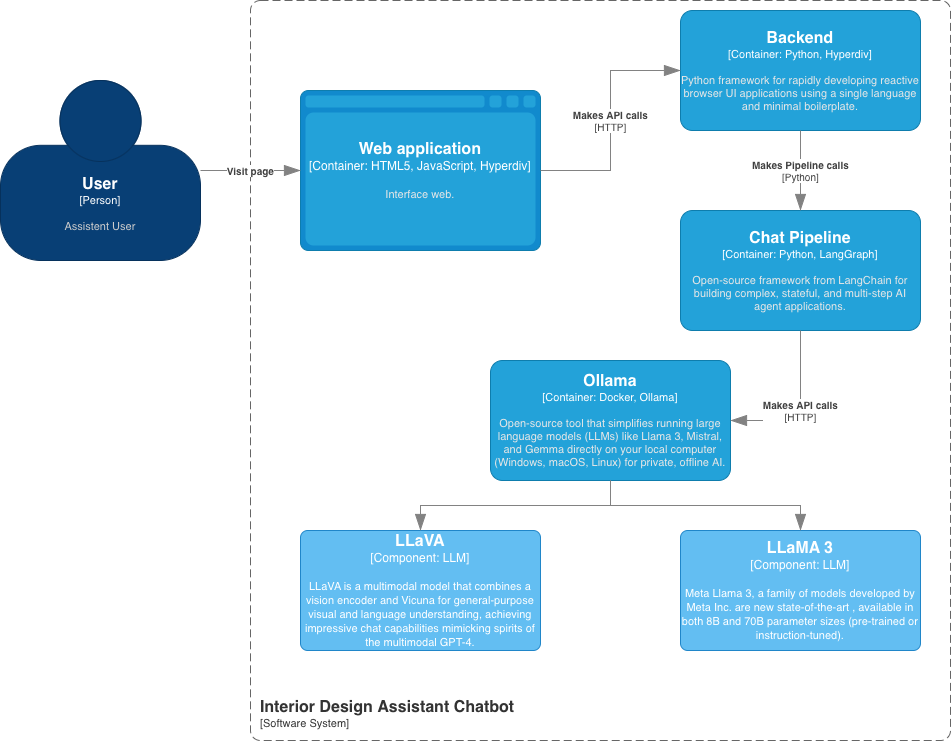
\includegraphics[scale=0.3]{images/c4-system-component.png}
            \caption{Diagrama C4 de Componente.}
         \end{figure}
        
        \subsection{Interface de Utilizador (\textit{Front-end})}
        Foi desenvolvida uma interface web minimalista utilizando a biblioteca Hyperdiv \cite{hyperdiv}. Esta interface foi desenhada para proporcionar uma interação fluida, oferecendo as seguintes funcionalidades:
        
        Gestão de Mensagens: Envio de instruções de texto e visualização do histórico de conversação.
        
        Interação Multimodal: Suporte para anexar ficheiros de imagem, permitindo que o modelo analise o contexto visual do ambiente.
        
        Controlo de Sessão: Opção para limpar o histórico de mensagens e reiniciar o estado da interação.

        \subsection{Arquitetura do \textit{Back-end }e Fluxo de Execução}
        O núcleo da aplicação reside no back-end, onde cada interação do utilizador é processada por um agente inteligente. A lógica de execução é orquestrada através de uma pipeline construída com a biblioteca LangGraph \cite{langgraph}, que permite definir o comportamento do agente como um grafo cíclico de estados.
        
        Ao submeter uma mensagem na interface, os dados são direcionados para o agente, cuja execução está organizada em quatro nós principais:
        \begin{enumerate}
            \item \textbf{Roteador:} Este nó atua como o ponto de entrada da pipeline e é responsável pela triagem dos dados submetidos pelo utilizador. A sua função primordial é verificar a presença de componentes multimodais na mensagem:
            \begin{itemize}
                \item \textbf{Deteção de Imagem:} Caso seja identificado um anexo de imagem, o fluxo é direcionado para o Nó Visual, onde será efetuado o processamento de visão computacional.
                \item \textbf{Fluxo Exclusivamente Textual:} Caso não seja detetada qualquer imagem, o sistema aciona o Nó Textual, otimizando o tempo de resposta ao ignorar as etapas de processamento visual desnecessárias.
            \end{itemize}
            Esta lógica de ramificação garante que o agente utilize o modelo mais adequado para o tipo de dado recebido, assegurando uma gestão eficiente dos recursos computacionais.
            \item \textbf{Textual:} Este nó é ativado sempre que a entrada do utilizador consiste exclusivamente em texto. O processamento é delegado ao modelo LLaMA \cite{llama}, sendo a interação estruturada através de uma instrução de sistema (\textit{System Prompt}) rigorosa que define o comportamento e o domínio de atuação do agente.
            \begin{enumerate}
                \item \textbf{Configuração do Modelo e Diretrizes:} Para garantir a qualidade e a relevância das respostas, o modelo é instanciado com as seguintes diretrizes permanentes:
                \item \textbf{Persona Profissional:} Atuação exclusiva como assistente especializado em Design de Interiores.
                \item \textbf{Estruturação de Respostas:} Obrigatoriedade de fornecer conselhos práticos e profissionais, estruturados preferencialmente em listas ou passos numerados para facilitar a leitura.
                \item \textbf{Foco na Valorização:} Em cenários de potencial venda do imóvel, o modelo é instruído a priorizar intervenções de elevado impacto visual e custo controlado.
                \item \textbf{Localização Linguística:} Tradução e adaptação obrigatória de todos os outputs para português de Portugal.
                \item \textbf{Gestão de Contexto e Memória:} Uma característica fundamental deste nó é a manutenção da coerência conversacional. A cada nova interação, o sistema injeta o histórico completo da sessão atual na pipeline. Esta abordagem permite que o modelo possua memória de curto prazo, sendo capaz de compreender referências a mensagens anteriores e manter a continuidade lógica do diálogo.
            \end{enumerate}
            \item \textbf{Visual:} Este nó é ativado exclusivamente quando o utilizador partilha ficheiros de imagem. A sua função primordial é a transcrição visual, transformando o conteúdo gráfico em dados textuais detalhados que possam ser interpretados pelos nós subsequentes da pipeline.
            Diferente do nó textual, este componente opera de forma isolada no que diz respeito ao histórico de conversação. Para maximizar a velocidade de processamento e reduzir a carga computacional, o histórico de contexto não é enviado. O modelo foca-se estritamente na análise imediata da imagem fornecida, garantindo uma resposta ágil e objetiva.
            O modelo de visão é configurado com uma diretriz específica para assegurar a precisão da análise:
            \begin{itemize}
                \item \textbf{Foco Descritivo:} Atuar como um assistente de design cujo objetivo é listar e descrever todos os elementos visíveis na imagem (mobiliário, iluminação, cores, disposição espacial).
                \item \textbf{Finalidade Técnica:} O output gerado é desenhado para servir de base informativa para o refinamento de sugestões de design que ocorrerá na etapa seguinte.
            \end{itemize}
            A função deste nó não é fornecer o conselho final ao utilizador, mas sim converter a percepção visual em linguagem natural. Este "resumo visual" será posteriormente integrado com o contexto histórico no nó final, garantindo que as sugestões de otimização sejam tecnicamente fundamentadas no que foi efetivamente observado na fotografia.
            \item \textbf{Refinamento:} Este nó constitui a etapa final da pipeline e é ativado sequencialmente após o processamento do Nó Visual. A sua função crítica é a fusão de dados: combinar a descrição técnica da imagem com o histórico da conversação para gerar uma resposta final coerente e personalizada.
            Integração de Dados e Contexto: O diferencial deste nó reside na sua capacidade de contextualização. O sistema injeta a descrição textual gerada anteriormente através da variável \textit{\{image\_description\}}, permitindo que o modelo "compreenda" o que foi visto na imagem sem a necessidade de processar novamente o ficheiro gráfico. O modelo utiliza um conjunto de instruções (\textit{System Prompt}) focado na qualidade do output final:
            \begin{enumerate}
                \item \textbf{Profissionalismo e Clareza:} O foco principal é a melhoria da clareza e do tom profissional dos conselhos de design de interiores.
                \item \textbf{Estruturação Lógica:} Tal como no nó textual, privilegia-se a organização da informação em listas ou passos numerados.
                \item \textbf{Estratégia de Valorização:} Reitera-se a prioridade em mudanças de elevado impacto e custo razoável para objetivos de valorização imobiliária.
                \item \textbf{Finalização Linguística:} Garante que a síntese final entre a análise da imagem e os conselhos teóricos seja entregue integralmente em português de Portugal.
            \end{enumerate}
            Ao consolidar a descrição visual com as intenções do utilizador (presentes no histórico), este nó assegura que as sugestões não são apenas genéricas, mas sim diretamente aplicáveis ao ambiente fotografado. O resultado é uma resposta refinada que encerra o ciclo de processamento do agente.
        \end{enumerate}

        Para uma melhor compreensão da dinâmica de execução e das ramificações de decisão do sistema, apresenta-se a figura \ref{fig:diagrama_fluxo} com o fluxograma do agente de conversação. Este diagrama ilustra a orquestração entre os nós de decisão (roteador), processamento de visão e refinamento textual, evidenciando como o estado é gerido ao longo da pipeline do LangGraph \cite{langgraph}.

        \begin{figure}[!h]
            \centering
            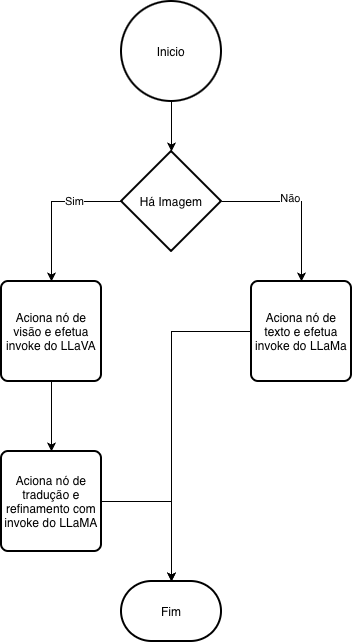
\includegraphics[scale=0.5]{images/diagrama-fluxo.png}
            \caption{Diagrama de Fluxo do Agente do Chat.}
            \label{fig:diagrama_fluxo}
        \end{figure}

        \subsection{Sequenciamento dos Agentes}

        A figura \ref{fig:diagrama_texto} contém o diagrama de sequência  seguinte ilustra o fluxo de execução quando o utilizador submete uma consulta exclusivamente textual. Este processo destaca a natureza síncrona da comunicação e a recuperação do histórico para garantir a continuidade do contexto.

        \begin{figure}[!h]
            \centering
            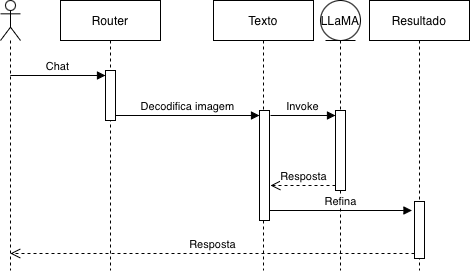
\includegraphics[scale=0.7]{images/diagrama-sequencia-texto.png}
            \caption{Diagrama de Sequencia de acionamento textual.}
            \label{fig:diagrama_texto}
         \end{figure}

        A figura \ref{fig:diagrama_visual} contém fluxo de execução para mensagens que contêm anexos de imagem é mais complexo, exigindo uma orquestração em várias etapas para garantir que o contexto visual seja corretamente interpretado e integrado na resposta final.

        \begin{figure}[!h]
            \centering
            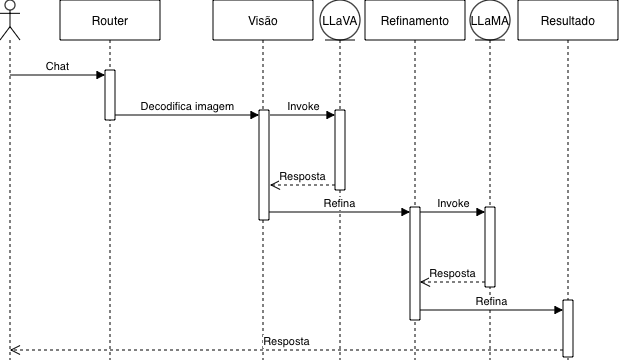
\includegraphics[scale=0.7]{images/diagrama-sequencia-visao.png}
            \caption{Diagrama de Fluxo de acionamento visual.}
            \label{fig:diagrama_visual}
         \end{figure}

         \subsection{Respositório do Código}
         Para efeitos de reprodutibilidade e análise detalhada da implementação, o repositório contendo o código deste trabalho está alojado no GitHub em: https://github.com/diegojeffersonms/IIA

%==========================================================================
% END DESENVOLVIMENTO
%==========================================================================

%==========================================================================
% BEGIN RESULTADOS E AVALIAÇÃO
%==========================================================================

\chapter{Resultados e Avaliação}
    \section{Resultados}
        Os testes realizados demonstraram que o assistente inteligente apresenta um comportamento robusto e alinhado com os objetivos propostos. A análise dos resultados foca-se na eficácia funcional e no desempenho técnico do sistema.

        \begin{figure}[!h]
            \centering
            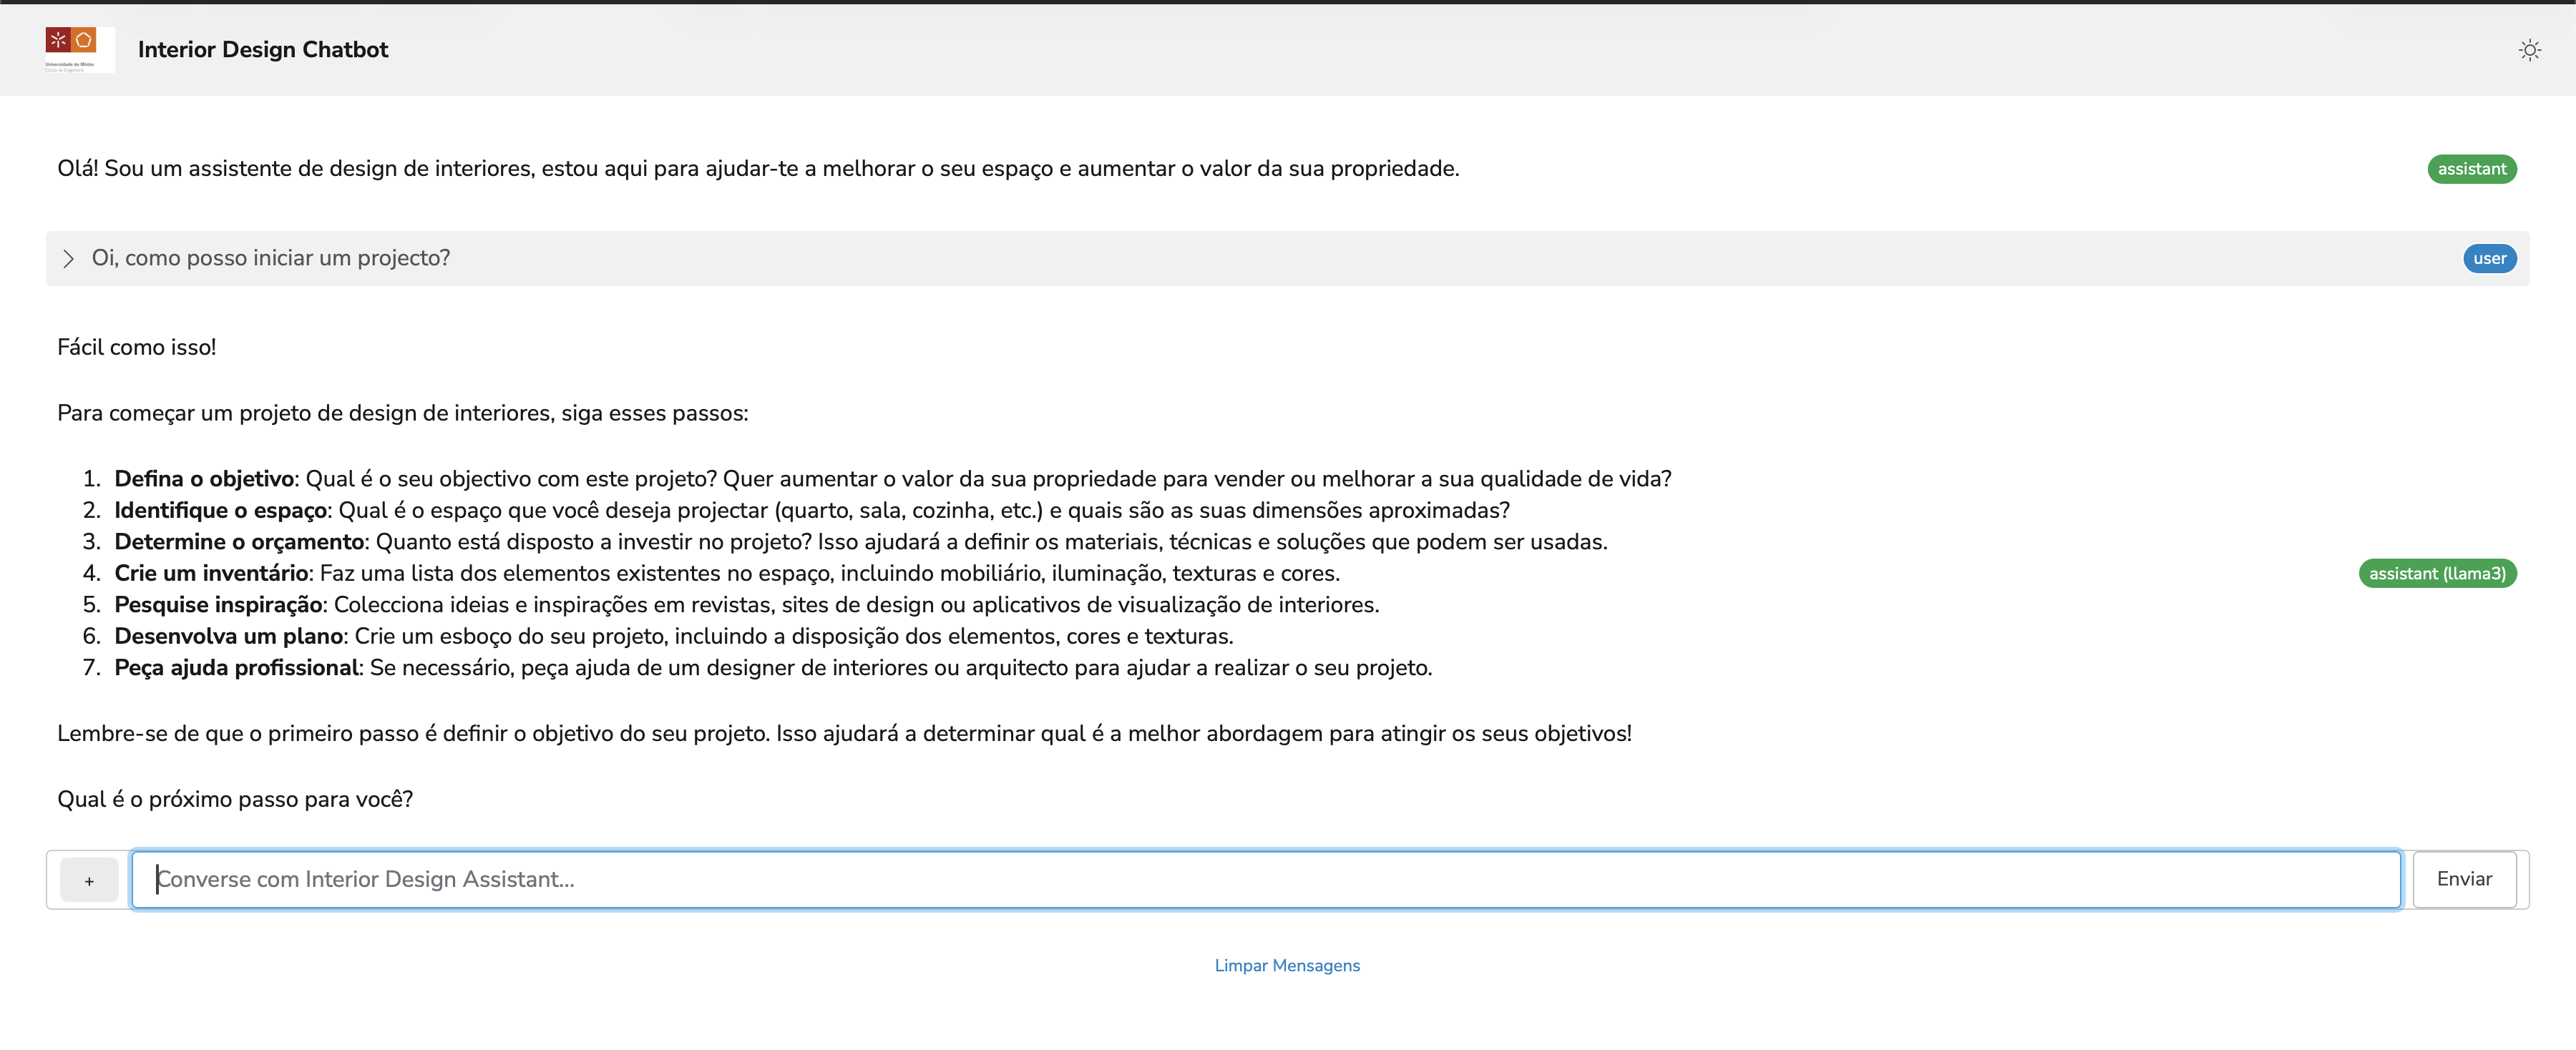
\includegraphics[scale=0.2]{images/chat-textual.png}
            \caption{Uso do Chat com Somente Texto.}
            \label{fig:chat_textual}
        \end{figure}

        \begin{figure}[!h]
            \centering
            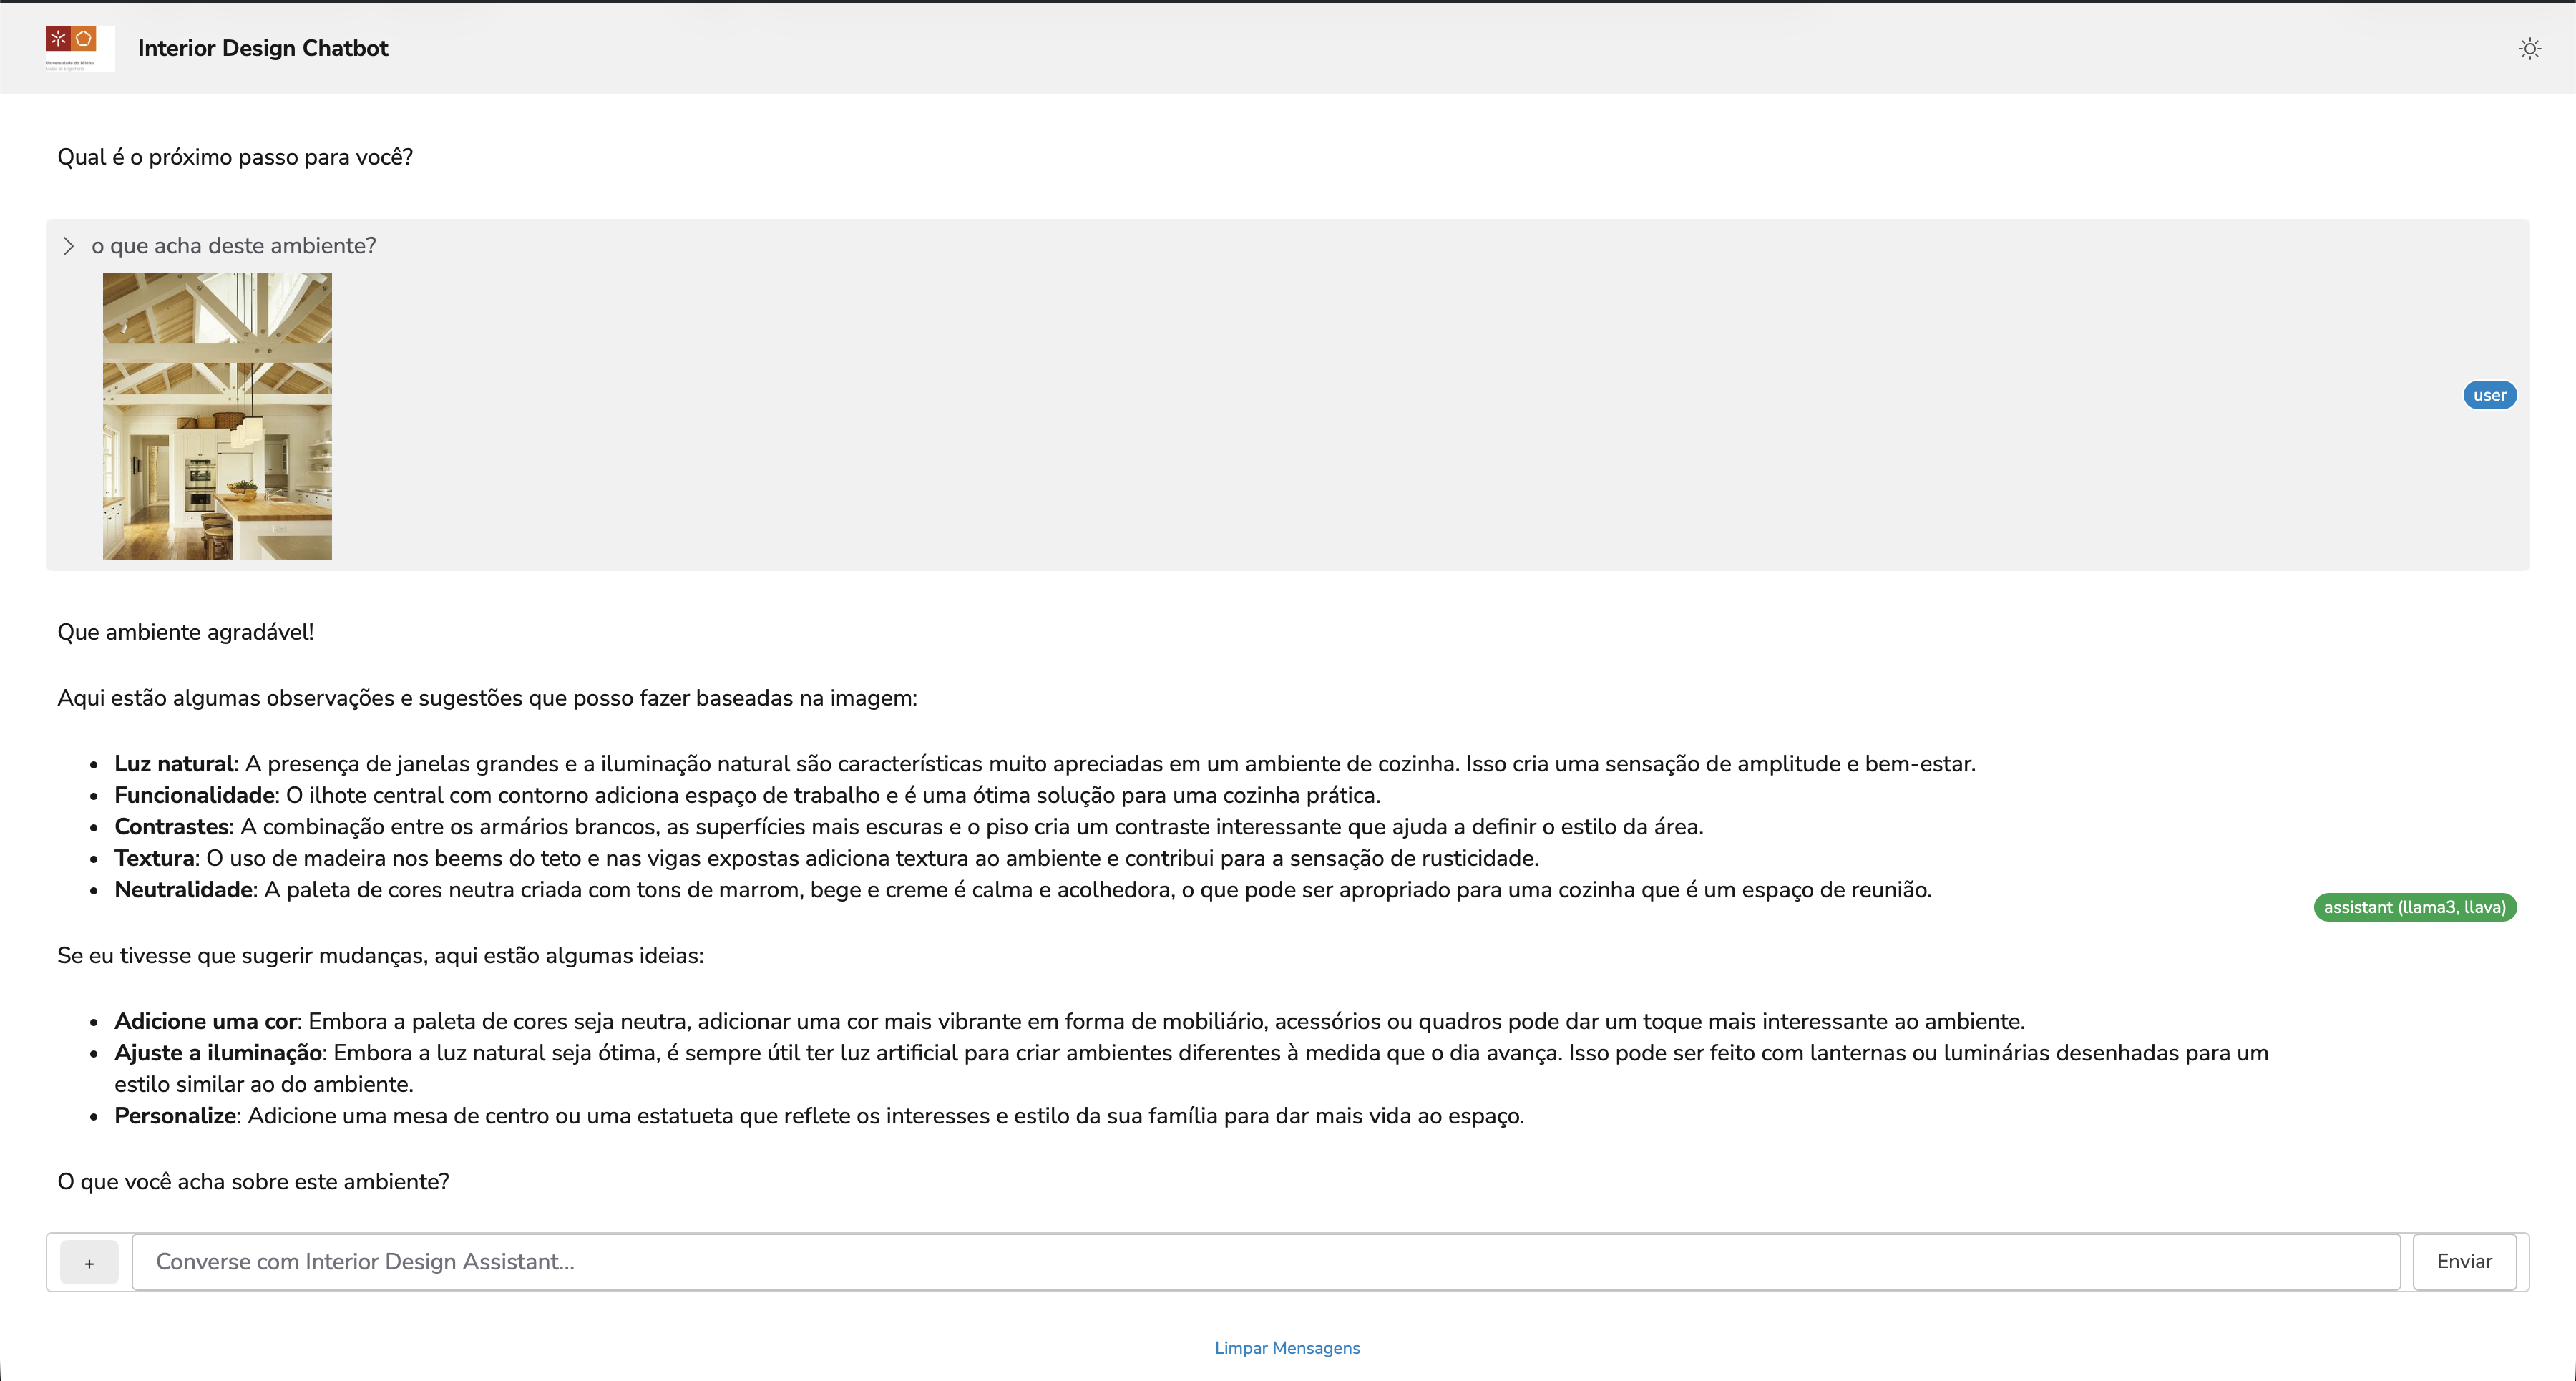
\includegraphics[scale=0.2]{images/chat-visual.png}
            \caption{Uso do Chat com Imagem e Texto.}
            \label{fig:chat_visual}
        \end{figure}

        \subsection{Eficácia Funcional e Qualidade das Respostas}
        O chatbot exibiu uma elevada competência na interpretação de contextos específicos de design de interiores. Observou-se que o sistema foi capaz de:
        \begin{itemize}
            \item \textbf{Interpretação Multimodal:} Identificar corretamente elementos em imagens reais, convertendo-os em descrições textuais úteis para o aconselhamento.
            \item \textbf{Pertinência das Sugestões:} Fornecer recomendações logicamente estruturadas, respeitando as diretrizes de otimização de espaço e valorização imobiliária.
            \item \textbf{Manutenção de Contexto:} Responder adequadamente a sequências de perguntas, demonstrando uma gestão de histórico eficaz durante a sessão.
        \end{itemize}

        \subsection{Desempenho e Viabilidade Técnica}
        Embora o sistema se tenha revelado funcional, o desempenho foi condicionado pela infraestrutura de execução. Devido à utilização do Ollama \cite{ollama} em ambiente Docker \cite{docker} sem aceleração por GPU, registou-se uma latência considerável na geração de respostas. No entanto, este atraso não comprometeu a precisão do modelo, servindo como uma Prova de Conceito para fins acadêmicos bem-sucedido.

        \subsection{Potencial de Evolução}
        Os resultados indicam que a arquitetura baseada em agentes é altamente escalável. Identificou-se que a precisão e a profundidade das respostas podem ser significativamente potenciadas através da implementação de técnicas de RAG (\textit{Retrieval-Augmented Generation}). A integração de uma base de dados vetorial permitiria complementar o conhecimento do modelo com catálogos técnicos, normas de arquitetura ou tendências de mercado atualizadas, reduzindo a ocorrência de alucinações e aumentando a autoridade das sugestões prestadas.

    \section{Discussão Crítica}
        A avaliação do protótipo desenvolvido permitiu identificar pontos fulcrais sobre a aplicação de modelos de linguagem locais em contextos de design de interiores. A análise divide-se entre as competências demonstradas pelo sistema e as condicionantes técnicas inerentes à arquitetura escolhida.

        \subsection{Pontos Fortes e Eficácia do Sistema}
        O sistema demonstrou uma elevada competência na análise multimodal, validando a eficácia da arquitetura em grafos. A capacidade do nó de visão em traduzir elementos espaciais em texto permitiu que o assistente fornecesse conselhos contextuais pertinentes, aproximando-se da percepção humana.
        Ao nível da experiência de utilizador (UX), a implementação de uma interface reativa com suporte para streaming revelou-se crucial. Esta funcionalidade mitiga a percepção de espera, permitindo que o utilizador acompanhe a geração progressiva da resposta. Adicionalmente, o projeto destaca-se pela sua conformidade ética e privacidade. Ao processar todos os dados localmente via Ollama \cite{ollama}, o sistema adere aos princípios de IA Responsável, garantindo que imagens de espaços privados não são transmitidas para servidores de terceiros.

        \subsection{Limitações e Desafios Técnicos}
        Apesar dos resultados positivos, foram identificadas limitações que impactam a escalabilidade da solução:
        \begin{itemize}
            \item Observou-se um tempo de resposta significativo (entre 10 a 30 segundos) no processamento de imagens. Este atraso deve-se à elevada carga computacional exigida pelos modelos de visão em hardware local.
            \item Atualmente, a memória de sessão é volátil. A ausência de uma base de dados dedicada para o histórico de longo prazo implica que o estado da conversação se perca caso a página seja recarregada.
            \item A execução fluida do sistema impõe requisitos técnicos elevados (mínimo de 8GB a 16GB de RAM), o que pode limitar a acessibilidade da ferramenta em dispositivos menos potentes.
        \end{itemize}

        \subsection{Análise Comparativa: Local vs. \textit{Cloud}}
        Comparando esta abordagem com o uso de modelos via API (como o GPT-4o da OpenAI), nota-se um \textit{trade-off} claro. Enquanto uma solução baseada na cloud ofereceria menor latência e uma base de conhecimento mais vasta, comprometeria a soberania de dados e a privacidade das imagens dos utilizadores, além de introduzir custos variáveis por utilização. O modelo local adotado neste trabalho posiciona-se como uma "caixa-preta" segura e privada, priorizando a segurança em detrimento da velocidade instantânea.

%==========================================================================
% END RESULTADOS E AVALIAÇÃO
%==========================================================================

%==========================================================================
% BEGIN CONCLUSÕES DE TRABALHO FUTURO
%==========================================================================

\chapter{Conclusões e Trabalho Futuro}
    O presente trabalho permitiu demonstrar a viabilidade e o potencial da aplicação de Inteligência Artificial Generativa na democratização do acesso a serviços de design de interiores e otimização habitacional. Através do desenvolvimento de um agente inteligente multimodal, foi possível responder à crescente necessidade de maximização de espaços em contextos urbanos de elevada densidade.
    A arquitetura implementada, baseada na orquestração de grafos de estado com o LangGraph \cite{langgraph} e na execução local de modelos via Ollama \cite{ollama}, revelou-se uma escolha técnica sólida. Esta abordagem não só garantiu a flexibilidade necessária para gerir fluxos complexos (texto e imagem), como também assegurou a total privacidade e soberania dos dados dos utilizadores, um fator crítico quando se lida com registos visuais de ambientes privados.
    Apesar das limitações identificadas ao nível da latência — decorrentes da execução em hardware sem aceleração dedicada (GPU) — o projeto atingiu com sucesso o estatuto de Prova de Conceito (PoC). O ChatBot demonstrou uma capacidade notável de interpretação visual e raciocínio lógico, fornecendo sugestões pertinentes e personalizadas que cumprem o objetivo de valorização funcional e patrimonial dos imóveis.
    
    \subsection{Trabalhos Futuros}
    Como perspetiva de evolução, este projeto estabelece os alicerces para implementações mais sofisticadas. Sugere-se para investigações futuras:
    \begin{itemize}
        \item Implementação de RAG (Retrieval-Augmented Generation) com uso de bases de dados externas para garantir que o assistente utiliza conhecimentos técnicos e normativas arquitetónicas atualizadas.
        \item Persistência de Longo Prazo com desenvolvimento de uma camada de base de dados para manter o histórico entre sessões, permitindo um acompanhamento contínuo de projetos de renovação.
    \end{itemize}
    Em suma, este trabalho evidencia que a IA, quando estruturada de forma modular e ética, pode atuar como uma ferramenta poderosa de apoio à decisão, transformando desafios demográficos e imobiliários em oportunidades de inovação tecnológica.

%==========================================================================
% END CONCLUSÕES DE TRABALHO FUTURO
%==========================================================================

%==========================================================================
% BEGIN REFERÊNCIAS
%==========================================================================

%% Changes biblibography name
%% Portuguese babel default : "Bibliografia"
%% Personally I prefer "Referências"
\renewcommand\bibname{Referências}

%% https://www.overleaf.com/learn/latex/bibliography_management_with_bibtex
\begin{thebibliography}{9}
\bibitem{ollama}
OLLAMA (2024). Ollama: Get up and running with large language models. [Online]. Disponível em: https://ollama.com [Acedido em: 11 de janeiro de 2026].
\bibitem{llava}
YOUNG, H. et al. (2023). LLaVA: Large Language and Vision Assistant. [Online]. Disponível em: https://llava-vl.github.io [Acedido em: 11 de janeiro de 2026].
\bibitem{llama}
META AI (2024). Introducing Llama 3: The most capable openly available LLM to date. [Online]. Disponível em: https://ai.meta.com/blog/meta-llama-3/ [Acedido em: 11 de janeiro de 2026].
\bibitem{langgraph}
LANGCHAIN (2024). LangGraph: Building Language Agents with Graphs. [Online]. Disponível em: https://www.langchain.com/langgraph [Acedido em: 11 de janeiro de 2026].
\bibitem{hyperdiv}
STEFANOVIC, M. (2024). Hyperdiv: Reactive web UI framework for Python. [Online]. Disponível em: https://hyperdiv.io [Acedido em: 11 de janeiro de 2026].
\bibitem{docker}
DOCKER (2024). Docker Documentation. [Online]. Disponível em: https://docs.docker.com [Acedido em: 11 de janeiro de 2026].
\end{thebibliography}

%==========================================================================
% END REFERÊNCIAS
%==========================================================================

%==========================================================================
% BEGIN LISTA DE SIGLAS E ACRÓNIMOS
%==========================================================================

%% Portuguese babel does not translate this environment
\renewcommand{\nomname}{Lista de Siglas e Acrónimos}

%% acronyms
\nomenclature[01]{\textbf{IA}}{Inteligência Artificial}
\nomenclature[02]{\textbf{LLM}}{\textit{Large Language Model} - Modelo de Linguagem Grande}
\nomenclature[03]{\textbf{LLaMA}}{Modelo de linguagem de texto da Meta}
\nomenclature[04]{\textbf{LLaVA}}{\textit{Large Language and Vision Assistant} - Modelo multimodal}
\nomenclature[05]{\textbf{GPU}}{\textit{Graphic Process Unit} - Unidade de Processamento Gráfico}
\nomenclature[06]{\textbf{PoC}}{\textit{Proof of Concept} - Prova de Conceito}
\nomenclature[07]{\textbf{RAG}}{\textit{Retrieval-Augmented Generation} - Geração Aumentada via Recuperação}
\nomenclature[08]{\textbf{API}}{\textit{Application Programming Interface} - Interface de Programação de Aplicação}
\nomenclature[09]{\textbf{RAM}}{\textit{Random Access Memory} - Memória de Acesso Aleatório (ou Randómico)}
\nomenclature[10]{\textbf{GB}}{\textit{Gigabyte} - uma unidade de medida de armazenamento ou memória}
\nomenclature[11]{\textbf{UX}}{\textit{User Experience} - Experiência do Usuário}
\nomenclature[12]{\textbf{TF-IDF}}{\textit{Term Frequency–Inverse Document Frequency} - Frequência do Termo–Inverso da Frequência}
\nomenclature[13]{\textbf{QA}}{\textit{Quality Assurance} - Garantia de Qualidade}

%% Show acronyms
\printnomenclature

%==========================================================================
% END LISTA DE SIGLAS E ACRÓNIMOS
%==========================================================================

%==========================================================================
% BEGIN ANEXOS
%==========================================================================

%% Why \addchap, instead of \chapter? 
%% \addchap has no numbering but appears in table of contents.
%% \addchap{Anexos}

%%     <<Os anexos deverão ser utilizados para a inclusão de informação adicional necessária para uma melhor compreensão do relatório o para complementar tópicos, secções ou assuntos abordados. Os anexos criados deverão ser numerados e possuir uma designação. Estes dados permitirão complementar o Índice geral do relatório relativamente à enumeração e apresentação dos diversos anexos.>>
    
    %% section version of \addchap
%%     \addsec{Anexo 1}


%==========================================================================
% END ANEXOS
%==========================================================================
\end{document}